\documentclass{article}%You can define the type of paper here.
%%Useful packages that I commonly use.
\usepackage[numbers]{natbib}%Bibliography package (help at http://merkel.zoneo.net/Latex/natbib.php).
\usepackage{url}%Package to highlight url.
\usepackage{times}%Sets font to be times.
\usepackage{alltt}%Allows the use of verbatim (good for printing out code).
\usepackage{graphicx}%Used to import images.
\usepackage{amsmath, amssymb, amscd}%Contains the AMS expanded math symbols library.
%%For those who want smaller margins, you can use this:
\usepackage[top=1in, bottom=1in, left=1in, right=1in]{geometry}
\usepackage{fancyhdr} %%For headers/footers
%\usepackage{savetrees} %%Removes white space
\pagestyle{fancy} %%For fancy headers
\usepackage{tocloft}
\renewcommand{\cftsecleader}{\cftdotfill{\cftdotsep}}
\usepackage{pdfpages}
\usepackage{morefloats}

\begin{document}

%% Top needs  to say "UNIVERSITY OF MONTANA: COMPUTER SCIENCE DEPARTMENT"
%%Title
\fancyhead[L]{UNIVERSITY OF MONTANA: COMPUTER SCIENCE DEPARTMENT} %%Header
\fancyfoot[L]{Blair Gemmer} %Left Footer
\fancyfoot[R]{CSCI 548 - Pattern Recognition} %Right Footer
\rhead{}
\renewcommand{\footrulewidth}{1pt}

%Fix headers on Table of Contents and List of Figures:
\fancypagestyle{plain}{
\fancyhead{}
\fancyfoot{}
\fancyhead[L]{UNIVERSITY OF MONTANA: COMPUTER SCIENCE DEPARTMENT} %%Header
\fancyfoot[L]{Blair Gemmer} %Left Footer
\fancyfoot[R]{CSCI 548 - Pattern Recognition} %Right Footer
\rhead{}
\renewcommand{\footrulewidth}{1pt}
}

%%Title
\title{Graduate Project:\\Visual Comparison of Edge Detection Algorithms}
\author{Blair Gemmer}
\maketitle


\newcommand*\Hide{%
\titleformat{\chapter}[display]
  {}{}{0pt}{\Huge}
\titleformat{\part}
  {}{}{0pt}{}
}

\newpage
%%Makes the paper use two columns
%\twocolumn

%%Table of Contents-------------------------------------------------------------------------------------

\tableofcontents


%%Introduction-------------------------------------------------------------------------------------
\section{Introduction}
\indent Running through the edge detection project, I noticed that there are a lot of different methods and algorithms for
 detecting edges. I decided to take a few choice algorithms, which are considered the most common methods -Sobel, 
Canny, LePlacian convolution mask, Gaussian convolution mask, Frei-Chen, Prewitt, Difference Edge Detection, and 
Homogeneity Edge Detection techniques- and test them using the human eye as a measure of goodness. I used 11 of
 the 3 most commonly detected images -4 images of fingerprints, 4 images of text, and 3 images  of faces- to run the 
techniques on and measure their goodness. I hope to find the best technique for each type of image and perhaps even
 the best technique overall.
\indent The benefits of finding the best edge detection algorithm will be that we will know what technique to use when
 faced with a specific problem among the 3 most commonly analyzed types of images.  
  

%%Method------------------------------------------------------------------------------------------
\section{Method}
The Sobel, Canny, Frei-Chen, Prewitt, Difference edge detection, and Homogeneity edge detection algorithms were all canned methods that were found in the biOps package for the R scripting language. The biOps package contains many methods and tools for image analysis and processing.

\indent For the programming portion of this project, I wrote a method to create and return a LePlacian mask. I wrote a method to return a weighted, normalized, distance matrix for the Gaussian mask. Then I wrote a method to iterate 
over each BLOB (Binary Large Object), which is a collection of pixels in an image matrix, and apply any given mask 
to the BLOB. I saved the pixel information in a copy of the image matrix and then returned the image matrix as an 
imagedata object. I wrote wrappers for each of the canned methods to maintain a standard method call for each. 
That way you can call $plotFreiChen(imageData)$, for example, and know that it will plot using the Frei-Chen 
algorithm, rather than having to remember to set $y = imgFreiChen(x), y=imgNegative(y), plot(y)$ which may 
be different syntax for each canned method. I finished by writing a method to plot using whichever algorithm is chosen
 as a parameter. The user can also choose to plot using all algorithms sequentially. I fixed a bug in my original project
 where the borders were showing up black instead of white using the LePlacian and/or the Gaussian masks. I also
 performed pre-processing on each of the images to maintain standards for image analysis. All images are RGB, .png, and each image is sized (keeping proportions) with their largest size being 500 pixels (either height or width).
 so the user doesn’t have to change anything in the script.

%%Results------------------------------------------------------------------------------------
\newpage
\section{Results}
The following are a series of 11 images that I ran through the 9 algorithms, for a total of 99 final images. The first image in each series is the original and each subsequent image will explain itself. 

\subsection{Fingerprint Recognition}

%Fingerprint:
\begin{figure}[h]
\centering
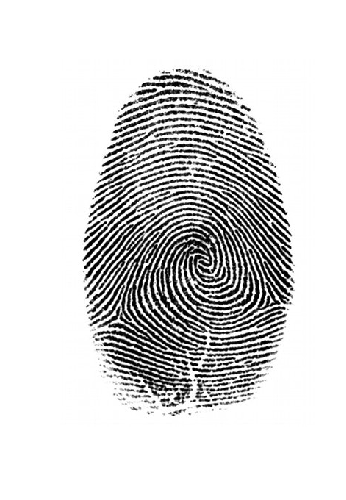
\includegraphics[scale=.85]{bigfinger.png}\\
{\bf Figure 1.0} Large fingerprint (Original)
\end{figure}  

\newpage
\begin{figure}[h]
\centering
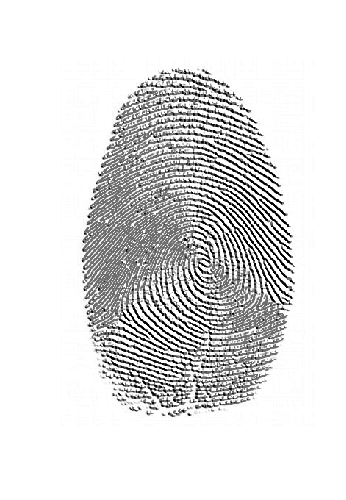
\includegraphics{bigfingerSobel.png}\\
{\bf Figure 1.1} Large fingerprint analyzed using the Sobel edge detection algorithm.   
\end{figure}


\newpage
\begin{figure}[h]
\centering
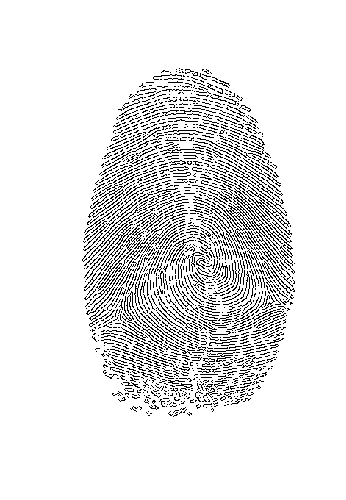
\includegraphics{bigfingerCanny.png}\\
{\bf Figure 1.2} Large fingerprint analyzed using the Canny edge detection algorithm.   
\end{figure}  

\newpage
\begin{figure}[h]
\centering
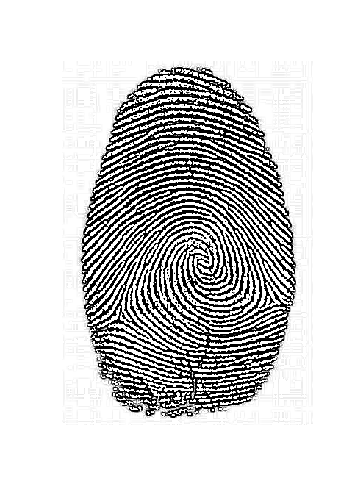
\includegraphics{bigfingerLePlace.png}\\
{\bf Figure 1.3} Large fingerprint analyzed using the LePlacian mask edge detection technique.  
\end{figure}  

\newpage
\begin{figure}[h]
\centering
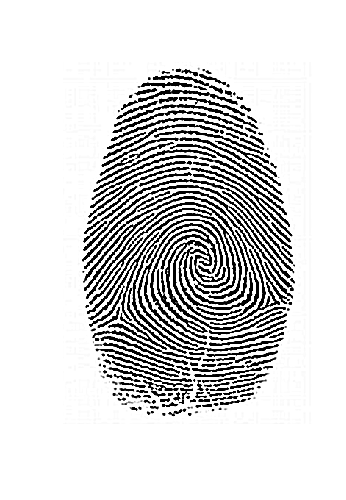
\includegraphics{bigfingerLePlaceGauss.png}\\
{\bf Figure 1.4} Large fingerprint analyzed using a Gaussian Mask and a LePlacian Mask in succession. Threshold = 0.   
\end{figure}  

\newpage
\begin{figure}[h]
\centering
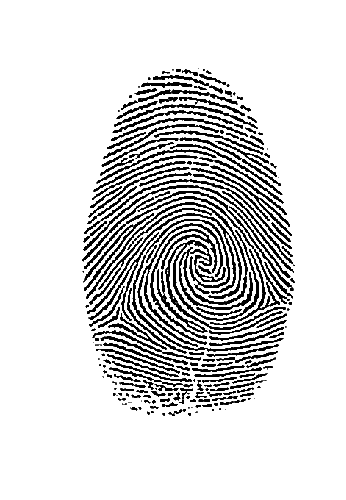
\includegraphics{bigfingerLePlaceGaussThreshold.png}\\
{\bf Figure 1.5} Large fingerprint analyzed using the LePlacian Gaussian mask technique with a threshold of 100.  
\end{figure}  

\newpage
\begin{figure}[h]
\centering
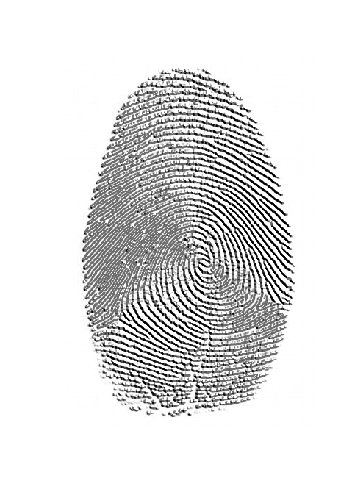
\includegraphics{bigfingerFreiChen.png}\\
{\bf Figure 1.6} Large fingerprint analyzed using the Frei-Chen edge detection algorithm.  
 \end{figure}  


\newpage
\begin{figure}[h]
\centering
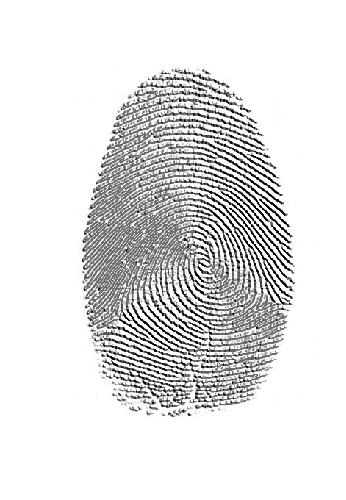
\includegraphics{bigfingerPrewitt.png}\\
{\bf Figure 1.7} Large fingerprint analyzed using the Prewitt edge detection algorithm.  
\end{figure}  
  
\newpage
\begin{figure}[h]
\centering
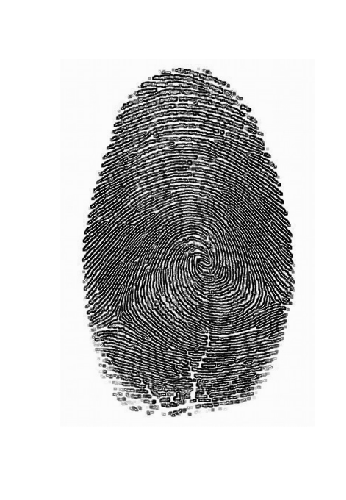
\includegraphics{bigfingerDiffEdge.png}\\
{\bf Figure 1.8} Large fingerprint analyzed using the Difference edge detection algorithm.  
\end{figure}    

\newpage
\begin{figure}[h]
\centering
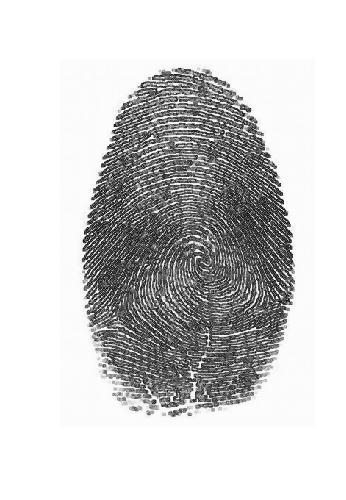
\includegraphics{bigfingerHomoEdge.png}\\  
{\bf Figure 1.9} Large fingerprint analyzed using the Homogeneity edge detection algorithm.  
\end{figure}  
 
\clearpage

 %Handprint:
\newpage
\begin{figure}[h]
\centering
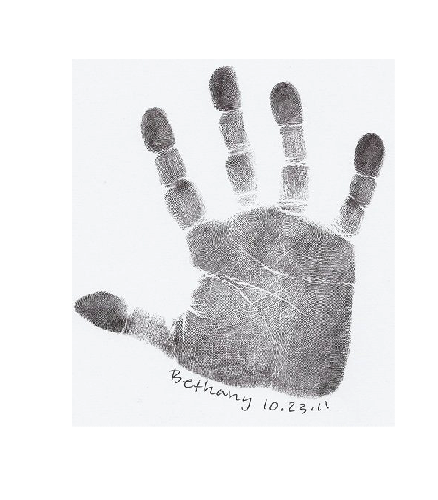
\includegraphics{handprint.png}\\
{\bf Figure 2.0} Handprint (Original)
\end{figure}

\newpage
\begin{figure}[h]
\centering
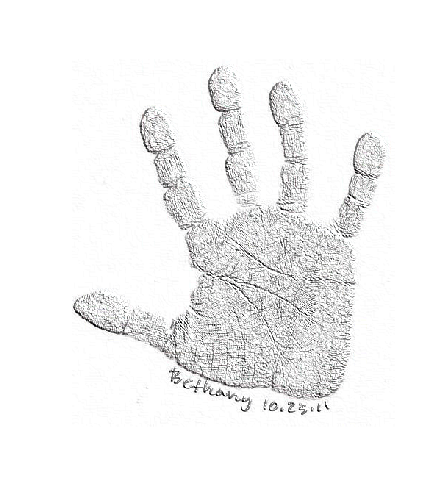
\includegraphics{handprintSobel.png}\\
{\bf Figure 2.1} Handprint analyzed using the Sobel edge detection algorithm.   
\end{figure}    
 
\newpage
\begin{figure}[h]
\centering
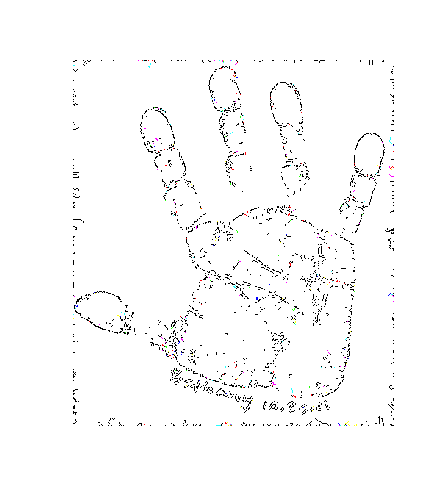
\includegraphics{handprintCanny.png}\\  
{\bf Figure 2.2} Handprint analyzed using the Canny edge detection algorithm.   
\end{figure}  
  
\newpage
\begin{figure}[h]
\centering
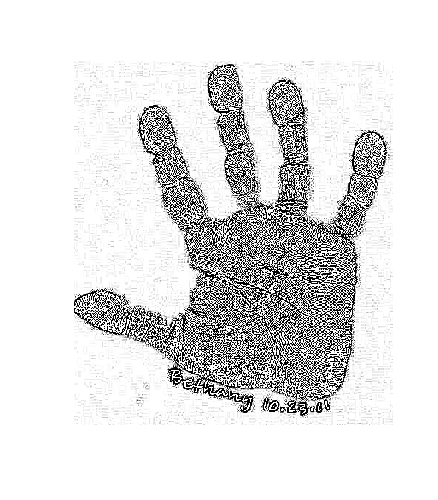
\includegraphics{handprintLePlace.png}\\
{\bf Figure 2.3} Handprint analyzed using the LePlacian mask edge detection algorithm.    
\end{figure}  
 
\newpage
\begin{figure}[h]
\centering
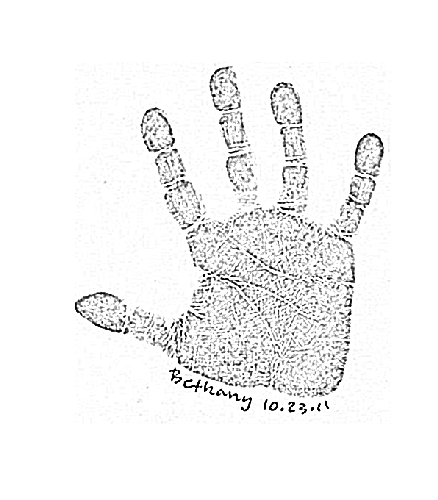
\includegraphics{handprintLePlaceGauss.png}\\
{\bf Figure 2.4} Handprint analyzed using a Gaussian Mask and a LePlacian Mask in succession. Threshold = 0.   
\end{figure}  

\newpage
\begin{figure}[h]
\centering
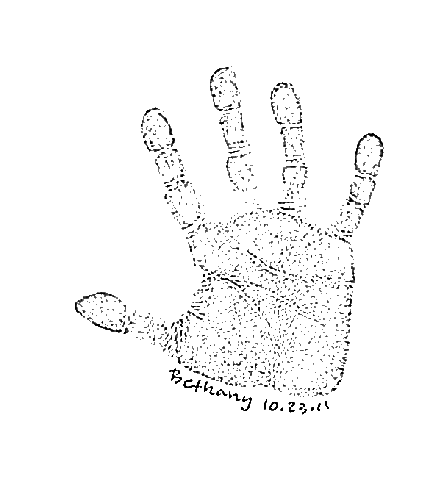
\includegraphics{handprintLePlaceGaussThreshold.png}\\
{\bf Figure 2.5} Handprint analyzed using the LePlacian-Gaussian mask algorithm with a threshold of 100.  
\end{figure}

\newpage
\begin{figure}[h]
\centering
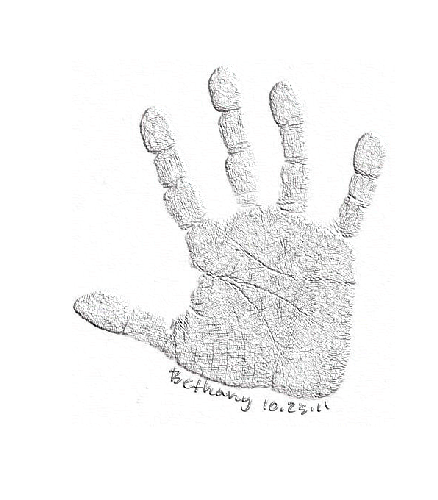
\includegraphics{handprintFreiChen.png}\\
{\bf Figure 2.6} Handprint analyzed using the Frei-Chen edge detection algorithm.  
\end{figure}


\newpage
\begin{figure}[h]
\centering
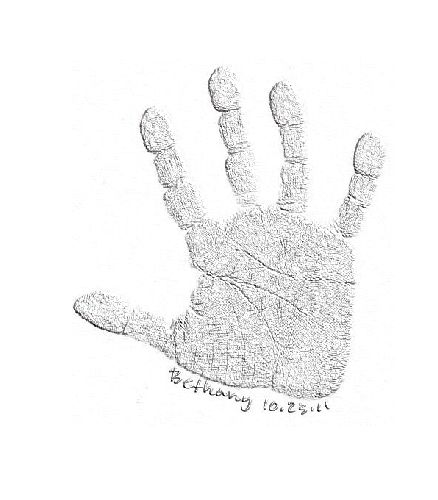
\includegraphics{handprintPrewitt.png}\\
{\bf Figure 2.7} Handprint analyzed using the Prewitt edge detection algorithm.  
\end{figure}

\newpage
\begin{figure}[h]
\centering
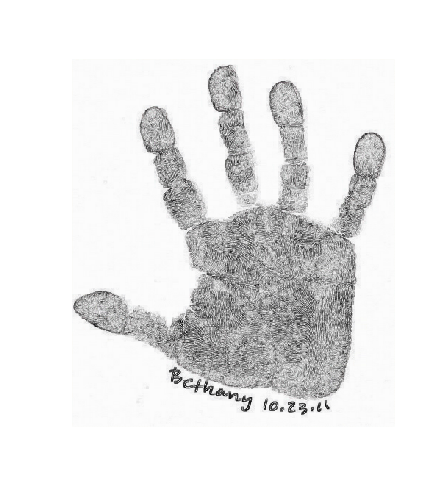
\includegraphics{handprintDiffEdge.png}\\
{\bf Figure 2.8} Handprint analyzed using the Difference edge detection algorithm.  
\end{figure}

\newpage
\begin{figure}[h]
\centering
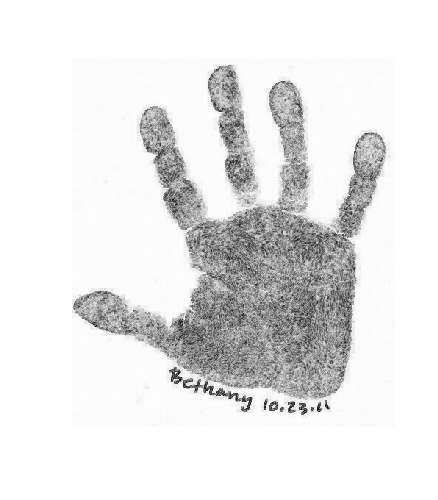
\includegraphics{handprintHomoEdge.png}\\
{\bf Figure 2.9} Handprint analyzed using the Homogeneity edge detection algorithm.  
\end{figure}  

\clearpage

%Dark Handprint:
\newpage
\begin{figure}[h]
\centering
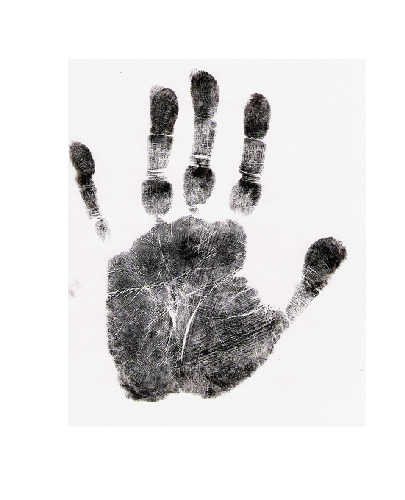
\includegraphics{darkhand.png}\\
{\bf Figure 3.0} Dark Handprint (Original)
\end{figure}

\newpage
\begin{figure}[h]
\centering
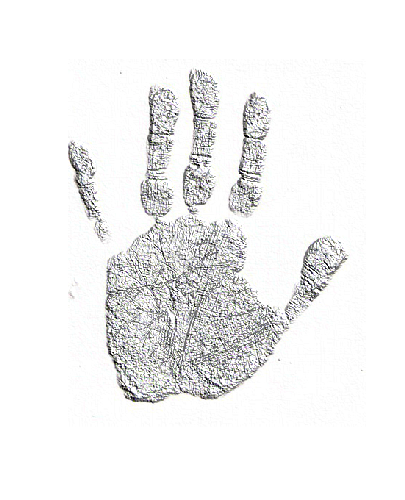
\includegraphics{darkhandSobel.png}\\
{\bf Figure 3.1} Dark Handprint analyzed using the Sobel edge detection algorithm. 
\end{figure}  

  

\newpage
\begin{figure}[h]
\centering
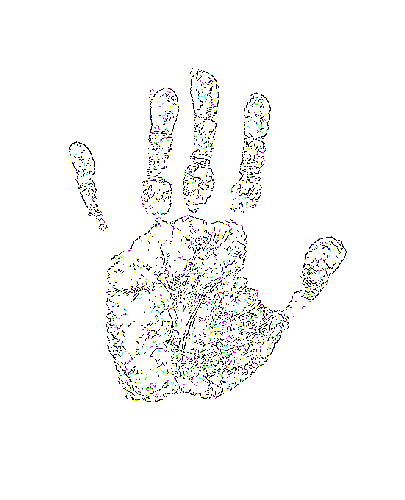
\includegraphics{darkhandCanny.png}\\
{\bf Figure 3.2} Dark Handprint analyzed using the Canny edge detection algorithm.   
\end{figure}

\newpage
\begin{figure}[h]
\centering
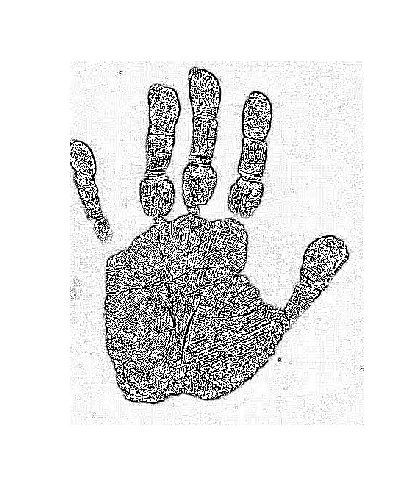
\includegraphics{darkhandLePlace.png}\\
{\bf Figure 3.3} Dark Handprint analyzed using the LePlacian mask edge detection algorithm.  
\end{figure}

\newpage
\begin{figure}[h]
\centering
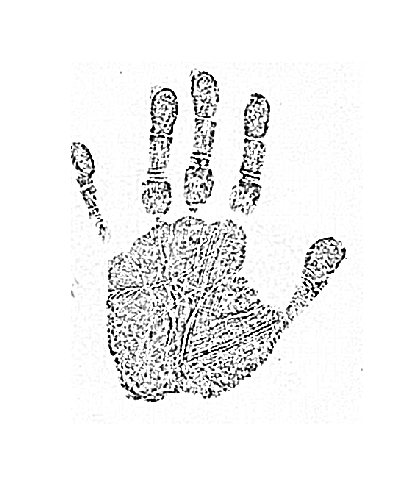
\includegraphics{darkhandLePlaceGauss.png}\\
{\bf Figure 3.4} Dark Handprint analyzed using a Gaussian Mask and a LePlacian Mask in succession. Threshold = 0.   
\end{figure}

\newpage
\begin{figure}[h]
\centering
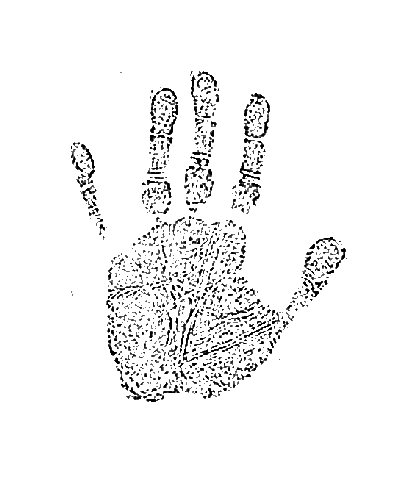
\includegraphics{darkhandLePlaceGaussThreshold.png}\\
{\bf Figure 3.5} Dark Handprint analyzed using the LePlacian-Gaussian mask algorithm with a threshold of 100.  
\end{figure}


\newpage
\begin{figure}[h]
\centering
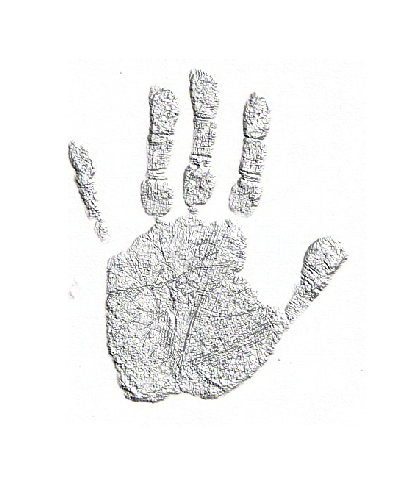
\includegraphics{darkhandFreiChen.png}\\
{\bf Figure 3.6} Dark Handprint analyzed using the Frei-Chen edge detection algorithm.  
\end{figure}

\newpage
\begin{figure}[h]
\centering
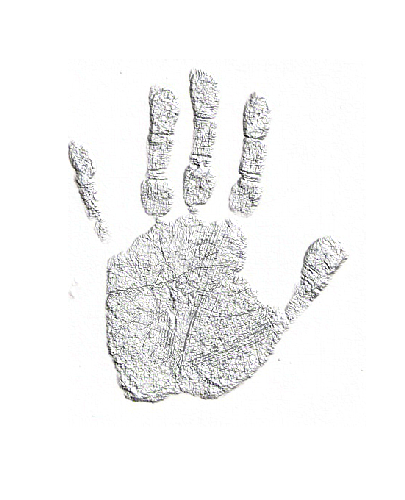
\includegraphics{darkhandPrewitt.png}\\
{\bf Figure 3.7} Dark Handprint analyzed using the Prewitt edge detection algorithm.  
\end{figure}

\newpage
\begin{figure}[h]
\centering
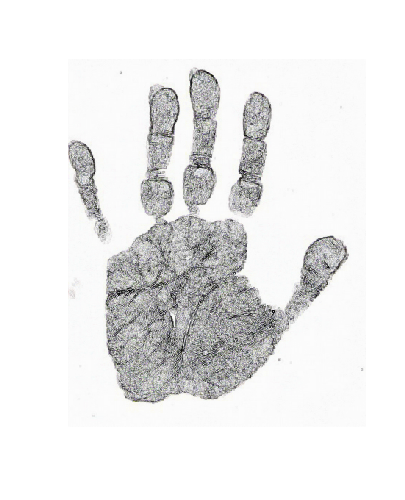
\includegraphics{darkhandDiffEdge.png}\\
{\bf Figure 3.8} Dark Handprint analyzed using the Difference edge detection algorithm.  
\end{figure}

\newpage
\begin{figure}[h]
\centering
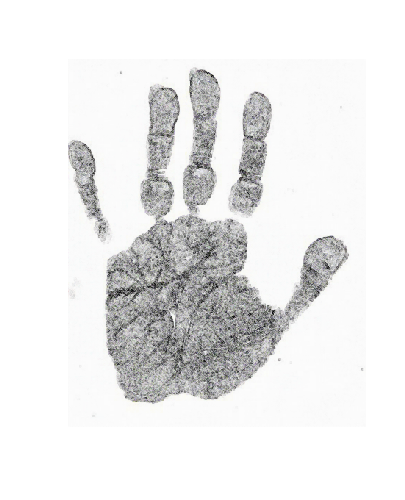
\includegraphics{darkhandHomoEdge.png}\\
{\bf Figure 3.9} Dark Handprint analyzed using the Homogeneity edge detection algorithm.  
\end{figure}

\clearpage

%Different Fingerprint Patterns:
\newpage
\begin{figure}[h]
\centering
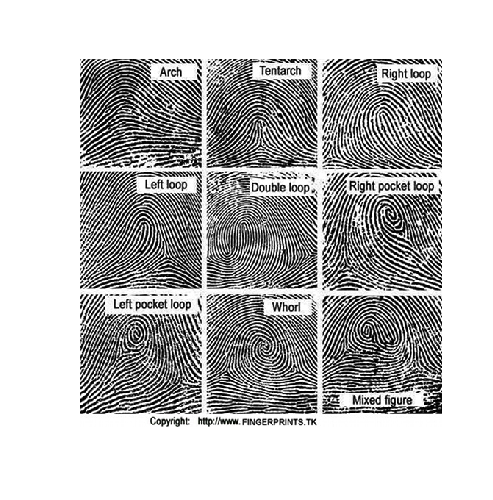
\includegraphics{patterns.png}\\
{\bf Figure 4.0} Different Fingerprint Patterns (Original)
\end{figure}

\newpage
\begin{figure}[h]
\centering
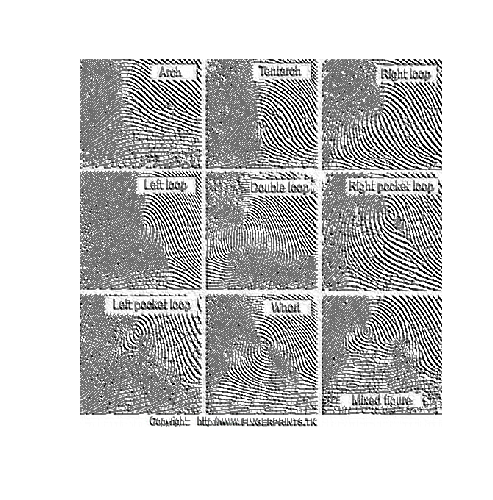
\includegraphics{patternsSobel.png}\\
{\bf Figure 4.1} Different Fingerprint Patterns analyzed using the Sobel edge detection algorithm.   
\end{figure}

\newpage
\begin{figure}[h]
\centering
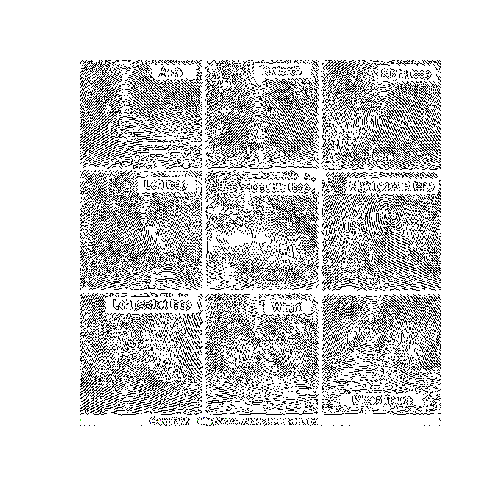
\includegraphics{patternsCanny.png}\\
{\bf Figure 4.2} Different Fingerprint Patterns analyzed using the Canny edge detection algorithm.   
\end{figure}

\newpage
\begin{figure}[h]
\centering
\includegraphics{patternsLeplace.png}\\
{\bf Figure 4.3} Different Fingerprint Patterns analyzed using the LePlacian mask edge detection algorithm.  
\end{figure}

\newpage
\begin{figure}[h]
\centering
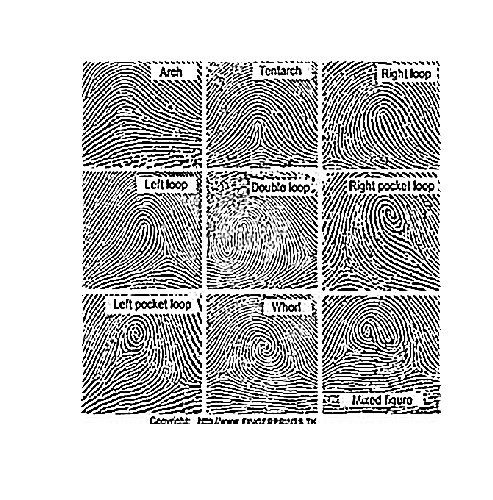
\includegraphics{patternsLePlaceGauss.png}\\
{\bf Figure 4.4} Different Fingerprint Patterns analyzed using a Gaussian Mask and a LePlacian Mask in succession. Threshold = 0.   
\end{figure}

\newpage
\begin{figure}[h]
\centering
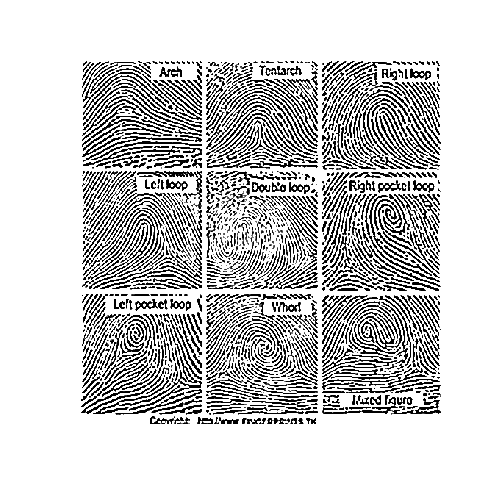
\includegraphics{patternsLePlaceGaussThreshold.png}\\
{\bf Figure 4.5} Different Fingerprint Patterns analyzed using the LePlacian-Gaussian mask algorithm with a threshold of 100.  
\end{figure}

\newpage
\begin{figure}[h]
\centering
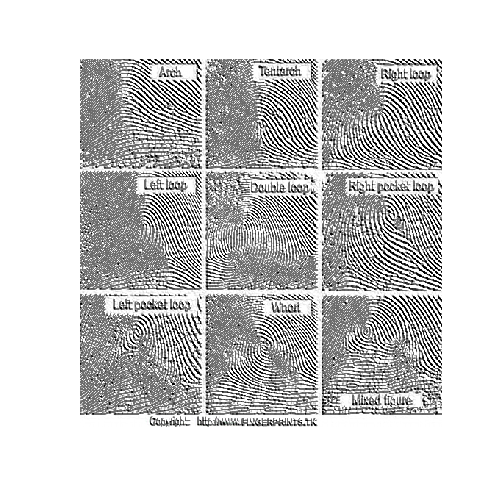
\includegraphics{patternsFreiChen.png}\\
{\bf Figure 4.6} Different Fingerprint Patterns analyzed using the Frei-Chen edge detection algorithm.  
\end{figure}

\newpage
\begin{figure}[h]
\centering
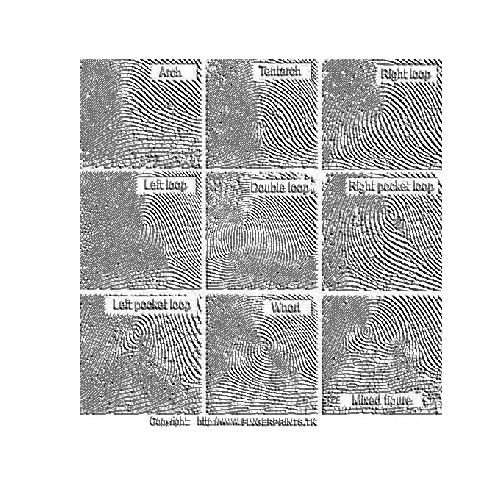
\includegraphics{patternsPrewitt.png}\\
{\bf Figure 4.7} Different Fingerprint Patterns analyzed using the Prewitt edge detection algorithm.  
\end{figure}

\newpage
\begin{figure}[h]
\centering
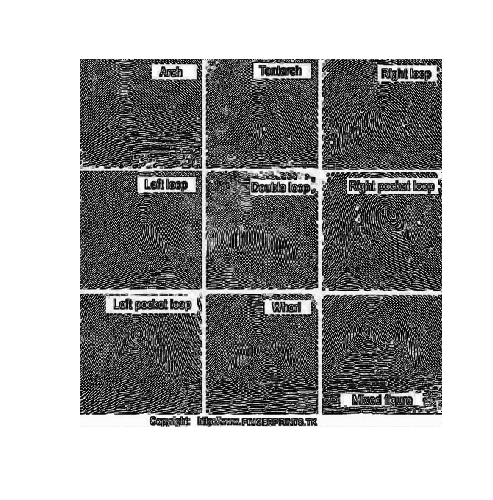
\includegraphics{patternsDiffEdge.png}\\
{\bf Figure 4.8} Different Fingerprint Patterns analyzed using the Difference edge detection algorithm.  
\end{figure}

\newpage
\begin{figure}[h]
\centering
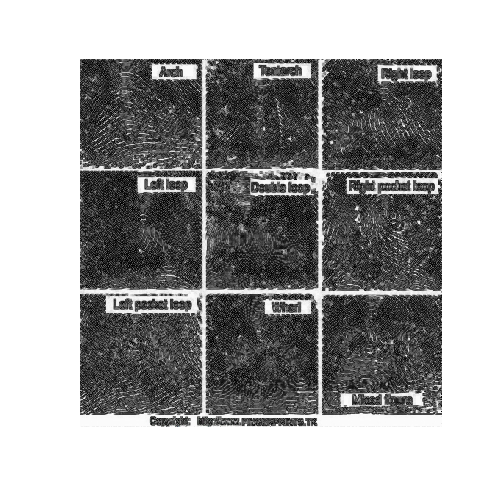
\includegraphics{patternsHomoEdge.png}\\
{\bf Figure 4.9} Different Fingerprint Patterns analyzed using the Homogeneity edge detection algorithm.  
\end{figure}

\clearpage

\subsection{Text Recognition}
%Normal Text:
\begin{figure}[h]
\centering
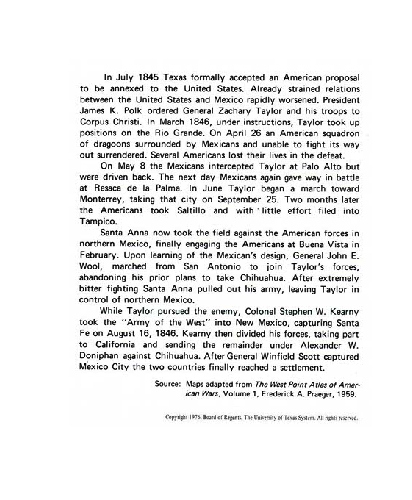
\includegraphics[scale=.85]{normaltext.png}\\
{\bf Figure 5.0} Normal Text (Original)
\end{figure}

\newpage
\begin{figure}[h]
\centering
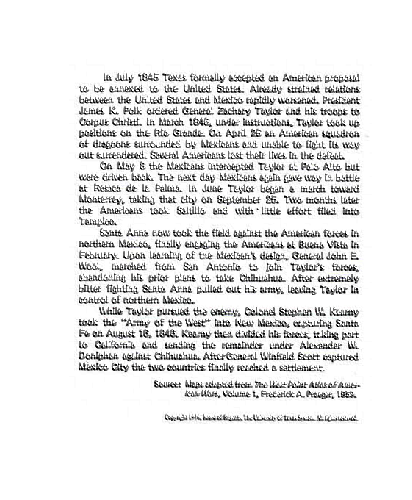
\includegraphics{normaltextSobel.png}\\
{\bf Figure 5.1} Normal Text analyzed using the Sobel edge detection algorithm.   
\end{figure}

\newpage
\begin{figure}[h]
\centering
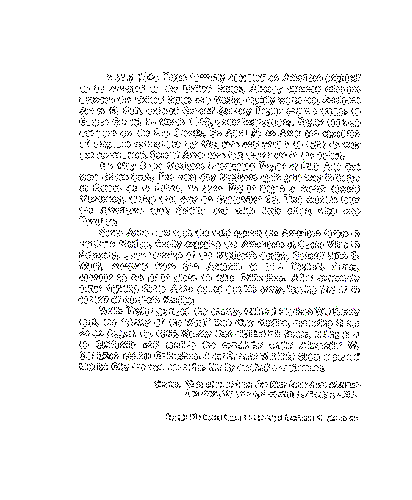
\includegraphics{normaltextCanny.png}\\
{\bf Figure 5.2} Normal Text analyzed using the Canny edge detection algorithm.   
\end{figure}

\newpage
\begin{figure}[h]
\centering
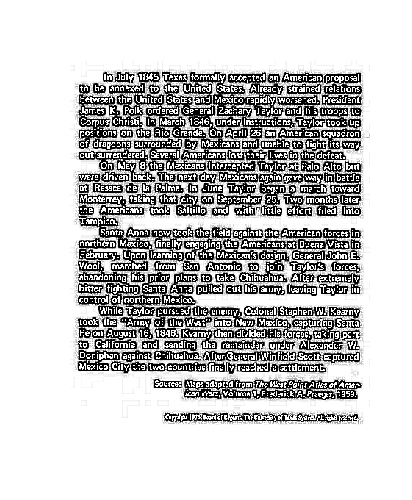
\includegraphics{normaltextLePlace.png}\\
{\bf Figure 5.3} Normal Text analyzed using the LePlacian mask edge detection algorithm.  
\end{figure}

\newpage
\begin{figure}[h]
\centering
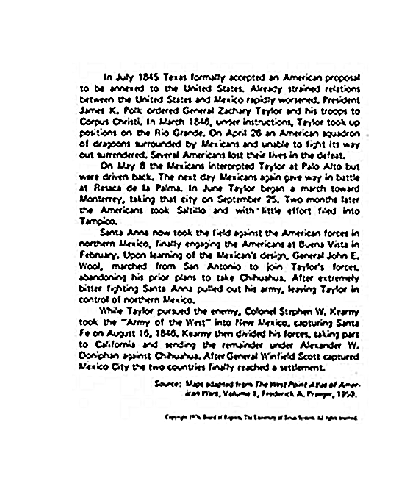
\includegraphics{normaltextLePlaceGauss.png}\\
{\bf Figure 5.4} Normal Text analyzed using a Gaussian Mask and a LePlacian Mask in succession. Threshold = 0.   
\end{figure}

\newpage
\begin{figure}[h]
\centering
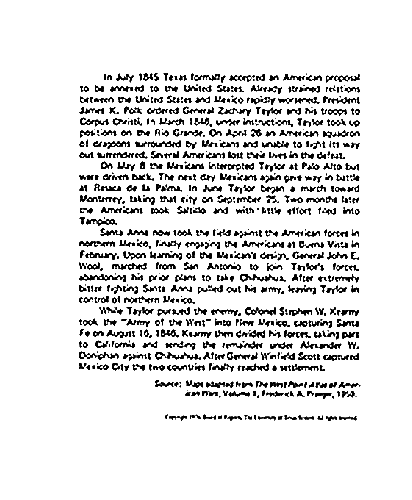
\includegraphics{normaltextLePlaceGaussThreshold.png}\\
{\bf Figure 5.5} Normal Text analyzed using the LePlacian-Gaussian mask algorithm with a threshold of 100.  
\end{figure}

\newpage
\begin{figure}[h]
\centering
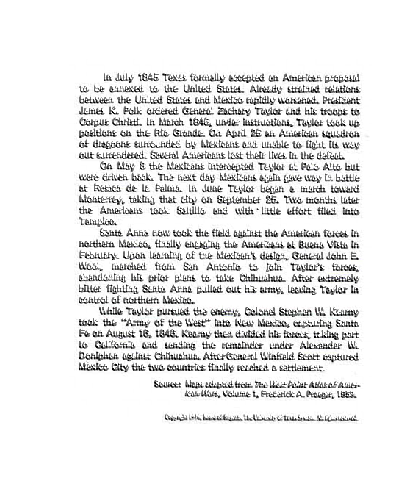
\includegraphics{normaltextFreiChen.png}\\
{\bf Figure 5.6} Normal Text analyzed using the Frei-Chen edge detection algorithm.  
\end{figure}

\newpage
\begin{figure}[h]
\centering
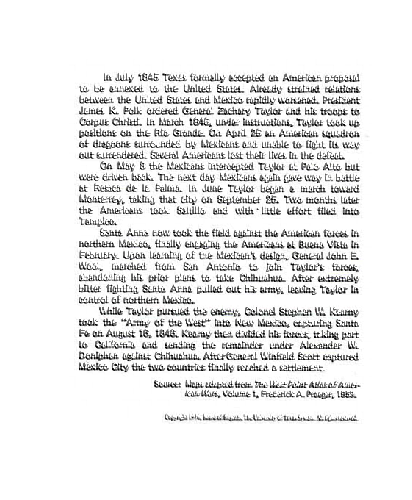
\includegraphics{normaltextPrewitt.png}\\
{\bf Figure 5.7} Normal Text analyzed using the Prewitt edge detection algorithm.  
\end{figure}

\newpage
\begin{figure}[h]
\centering
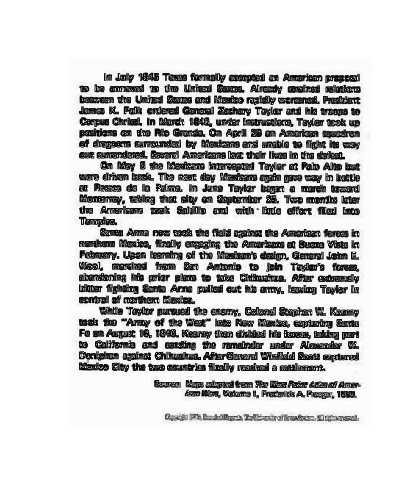
\includegraphics{normaltextDiffEdge.png}\\
{\bf Figure 5.8} Normal Text analyzed using the Difference edge detection algorithm.  
\end{figure}

\newpage
\begin{figure}[h]
\centering
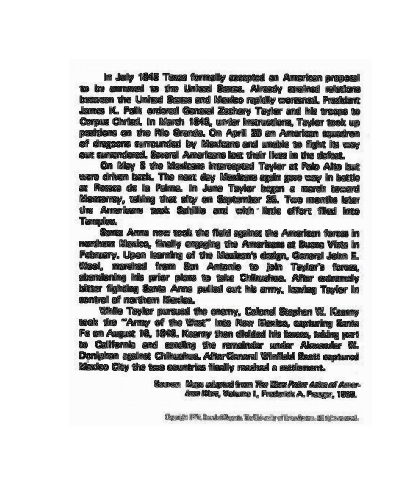
\includegraphics{normaltextHomoEdge.png}\\
{\bf Figure 5.9} Normal Text analyzed using the Homogeneity edge detection algorithm.  
\end{figure}

\clearpage


%Normal Text with Differing Font Sizes:
\newpage
\begin{figure}[h]
\centering
\includegraphics{diffnormal.png}\\
{\bf Figure 6.0} Normal Text with Differing Font Sizes (Original)
\end{figure}

\newpage
\begin{figure}[h]
\centering
\includegraphics{diffnormalSobel.png}\\
{\bf Figure 6.1} Normal Text with Differing Font Sizes analyzed using the Sobel edge detection algorithm.   
\end{figure}

\newpage
\begin{figure}[h]
\centering
\includegraphics{diffnormalCanny.png}\\
{\bf Figure 6.2} Normal Text with Differing Font Sizes analyzed using the Canny edge detection algorithm.   
\end{figure}

\newpage
\begin{figure}[h]
\centering
\includegraphics{diffnormalLePlace.png}\\
{\bf Figure 6.3} Normal Text with Differing Font Sizes analyzed using the LePlacian mask edge detection algorithm.  
\end{figure}

\newpage
\begin{figure}[h]
\centering
\includegraphics{diffnormalLePlaceGauss.png}\\
{\bf Figure 6.4} Normal Text with Differing Font Sizes analyzed using a Gaussian Mask and a LePlacian Mask in succession. Threshold = 0.   
\end{figure}

\newpage
\begin{figure}[h]
\centering
\includegraphics{diffnormalLePlaceGaussThreshold.png}\\
{\bf Figure 6.5} Normal Text with Differing Font Sizes analyzed using the LePlacian-Gaussian mask algorithm with a threshold of 100.  
\end{figure}

\newpage
\begin{figure}[h]
\centering
\includegraphics{diffnormalFreiChen.png}\\
{\bf Figure 6.6} Normal Text with Differing Font Sizes analyzed using the Frei-Chen edge detection algorithm.  
\end{figure}

\newpage
\begin{figure}[h]
\centering
\includegraphics{diffnormalPrewitt.png}\\
{\bf Figure 6.7} Normal Text with Differing Font Sizes analyzed using the Prewitt edge detection algorithm.  
\end{figure}

\newpage
\begin{figure}[h]
\centering
\includegraphics{diffnormalDiffEdge.png}\\
{\bf Figure 6.8} Normal Text with Differing Font Sizes analyzed using the Difference edge detection algorithm.  
\end{figure}

\newpage
\begin{figure}[h]
\centering
\includegraphics{diffnormalHomoEdge.png}\\
{\bf Figure 6.9} Normal Text with Differing Font Sizes analyzed using the Homogeneity edge detection algorithm.  
\end{figure}

\clearpage


%Weird Text with Differing Font Sizes:
\newpage
\begin{figure}[h]
\centering
\includegraphics{weirdtext.png}\\
{\bf Figure 7.0} Weird Text with Differing Font Sizes (Original)
\end{figure}

\newpage
\begin{figure}[h]
\centering
\includegraphics{weirdtextSobel.png}\\
{\bf Figure 7.1} Weird Text with Differing Font Sizes analyzed using the Sobel edge detection algorithm.   
\end{figure}

\newpage
\begin{figure}[h]
\centering
\includegraphics{weirdtextCanny.png}\\
{\bf Figure 7.2} Weird Text with Differing Font Sizes analyzed using the Canny edge detection algorithm.   
\end{figure}

\newpage
\begin{figure}[h]
\centering
\includegraphics{weirdtextLePlace.png}\\
{\bf Figure 7.3} Weird Text with Differing Font Sizes analyzed using the LePlacian mask edge detection algorithm.  
\end{figure}

\newpage
\begin{figure}[h]
\centering
\includegraphics{weirdtextLePlaceGauss.png}\\
{\bf Figure 7.4} Weird Text with Differing Font Sizes analyzed using a Gaussian Mask and a LePlacian Mask in succession. Threshold = 0.   
\end{figure}

\newpage
\begin{figure}[h]
\centering
\includegraphics{weirdtextLePlaceGaussThreshold.png}\\
{\bf Figure 7.5} Weird Text with Differing Font Sizes analyzed using the LePlacian-Gaussian mask algorithm with a threshold of 100.  
\end{figure}

\newpage
\begin{figure}[h]
\centering
\includegraphics{weirdtextFreiChen.png}\\
{\bf Figure 7.6} Weird Text with Differing Font Sizes analyzed using the Frei-Chen edge detection algorithm.  
\end{figure}

\newpage
\begin{figure}[h]
\centering
\includegraphics{weirdtextPrewitt.png}\\
{\bf Figure 7.7} Weird Text with Differing Font Sizes analyzed using the Prewitt edge detection algorithm.  
\end{figure}

\newpage
\begin{figure}[h]
\centering
\includegraphics{weirdtextDiffEdge.png}\\
{\bf Figure 7.8} Weird Text with Differing Font Sizes analyzed using the Difference edge detection algorithm.  
\end{figure}

\newpage
\begin{figure}[h]
\centering
\includegraphics{weirdtextHomoEdge.png}\\
{\bf Figure 7.9} Weird Text with Differing Font Sizes analyzed using the Homogeneity edge detection algorithm.  
\end{figure}

\clearpage


%Text with Differing Font Sizes and Differing Languages:
\newpage
\begin{figure}[h]
\centering
\includegraphics{thankyou.png}\\
{\bf Figure 8.0} Text with Differing Font Sizes and Differing Languages (Original)
\end{figure}


\newpage
\begin{figure}[h]
\centering
\includegraphics{thankyouSobel.png}\\
{\bf Figure 8.1} Text with Differing Font Sizes and Differing Languages analyzed using the Sobel edge detection algorithm.   
\end{figure}

\newpage
\begin{figure}[h]
\centering
\includegraphics{thankyouCanny.png}\\
{\bf Figure 8.2} Text with Differing Font Sizes and Differing Languages analyzed using the Canny edge detection algorithm.   
\end{figure}

\newpage
\begin{figure}[h]
\centering
\includegraphics{thankyouLePlace.png}\\
{\bf Figure 8.3} Text with Differing Font Sizes and Differing Languages analyzed using the LePlacian mask edge detection algorithm.  
\end{figure}

\newpage
\begin{figure}[h]
\centering
\includegraphics{thankyouLePlaceGauss.png}\\
{\bf Figure 8.4} Text with Differing Font Sizes and Differing Languages analyzed using a Gaussian Mask and a LePlacian Mask in succession. 
Threshold = 0. 
\end{figure}

\newpage
\begin{figure}[h]
\centering
\includegraphics{thankyouLePlaceGaussThreshold.png}\\
{\bf Figure 8.5} Text with Differing Font Sizes and Differing Languages analyzed using the LePlacian-Gaussian mask algorithm with a threshold of 100.  
\end{figure}

\newpage
\begin{figure}[h]
\centering
\includegraphics{thankyouFreiChen.png}\\
{\bf Figure 8.6} Text with Differing Font Sizes and Differing Languages analyzed using the Frei-Chen edge detection algorithm.  
\end{figure}

\newpage
\begin{figure}[h]
\centering
\includegraphics{thankyouPrewitt.png}\\
{\bf Figure 8.7} Text with Differing Font Sizes and Differing Languages analyzed using the Prewitt edge detection algorithm.  
\end{figure}

\newpage
\begin{figure}[h]
\centering
\includegraphics{thankyouDiffEdge.png}\\
{\bf Figure 8.8} Text with Differing Font Sizes and Differing Languages analyzed using the Difference edge detection algorithm.  
\end{figure}

\newpage
\begin{figure}[h]
\centering
\includegraphics{thankyouHomoEdge.png}\\
{\bf Figure 8.9} Text with Differing Font Sizes and Differing Languages analyzed using the Homogeneity edge detection algorithm.  
\end{figure}

\clearpage


\subsection{Face Recognition}
%Smiling Person:
\begin{figure}[h]
\centering
\includegraphics[scale=.85]{smiling.png}\\
{\bf Figure 9.0} Photo of Smiling Person (Original)
\end{figure}

\newpage
\begin{figure}[h]
\centering
\includegraphics{smilingSobel.png}\\
{\bf Figure 9.1} Photo of Smiling Person analyzed using the Sobel edge detection algorithm.   
\end{figure}

\newpage
\begin{figure}[h]
\centering
\includegraphics{smilingCanny.png}\\
{\bf Figure 9.2} Photo of Smiling Person analyzed using the Canny edge detection algorithm.   
\end{figure}

\newpage
\begin{figure}[h]
\centering
\includegraphics{smilingLePlace.png}\\
{\bf Figure 9.3} Photo of Smiling Person analyzed using the LePlacian mask edge detection algorithm.  
\end{figure}

\newpage
\begin{figure}[h]
\centering
\includegraphics{smilingLePlaceGauss.png}\\
{\bf Figure 9.4} Photo of Smiling Person analyzed using a Gaussian Mask and a LePlacian Mask in succession. Threshold = 0.   
\end{figure}

\newpage
\begin{figure}[h]
\centering
\includegraphics{smilingLePlaceGaussThreshold.png}\\
{\bf Figure 9.5} Photo of Smiling Person analyzed using the LePlacian-Gaussian mask algorithm with a threshold of 100.  
\end{figure}

\newpage
\begin{figure}[h]
\centering
\includegraphics{smilingFreiChen.png}\\
{\bf Figure 9.6} Photo of Smiling Person analyzed using the Frei-Chen edge detection algorithm.  
\end{figure}

\newpage
\begin{figure}[h]
\centering
\includegraphics{smilingPrewitt.png}\\
{\bf Figure 9.7} Photo of Smiling Person analyzed using the Prewitt edge detection algorithm.  
\end{figure}

\newpage
\begin{figure}[h]
\centering
\includegraphics{smilingDiffEdge.png}\\
{\bf Figure 9.8} Photo of Smiling Person analyzed using the Difference edge detection algorithm.  
\end{figure}

\newpage
\begin{figure}[h]
\centering
\includegraphics{smilingHomoEdge.png}\\
{\bf Figure 9.9} Photo of Smiling Person analyzed using the Homogeneity edge detection algorithm.  
\end{figure}

\clearpage


%Old Person:
\newpage
\begin{figure}[h]
\centering
\includegraphics{old.png}\\
{\bf Figure 10.0} Photo of Old Person (Original)
\end{figure}


\newpage
\begin{figure}[h]
\centering
\includegraphics{oldSobel.png}\\
{\bf Figure 10.1} Photo of Old Person analyzed using the Sobel edge detection algorithm.   
\end{figure}

\newpage
\begin{figure}[h]
\centering
\includegraphics{oldCanny.png}\\
{\bf Figure 10.2} Photo of Old Person analyzed using the Canny edge detection algorithm.   
\end{figure}

\newpage
\begin{figure}[h]
\centering
\includegraphics{oldLePlace.png}\\
{\bf Figure 10.3} Photo of Old Person analyzed using the LePlacian mask edge detection algorithm.  
\end{figure}

\newpage
\begin{figure}[h]
\centering
\includegraphics{oldLePlaceGauss.png}\\
{\bf Figure 10.4} Photo of Old Person analyzed using a Gaussian Mask and a LePlacian Mask in succession. Threshold = 0.   
\end{figure}

\newpage
\begin{figure}[h]
\centering
\includegraphics{oldLePlaceGaussThreshold.png}\\
{\bf Figure 10.5} Photo of Old Person analyzed using the LePlacian-Gaussian mask algorithm with a threshold of 100.  
\end{figure}

\newpage
\begin{figure}[h]
\centering
\includegraphics{oldFreiChen.png}\\
{\bf Figure 10.6} Photo of Old Person analyzed using the Frei-Chen edge detection algorithm.  
\end{figure}

\newpage
\begin{figure}[h]
\centering
\includegraphics{oldPrewitt.png}\\
{\bf Figure 10.7} Photo of Old Person analyzed using the Prewitt edge detection algorithm.  
\end{figure}

\newpage
\begin{figure}[h]
\centering
\includegraphics{oldDiffEdge.png}\\
{\bf Figure 10.8} Photo of Old Person analyzed using the Difference edge detection algorithm.  
\end{figure}

\newpage
\begin{figure}[h]
\centering
\includegraphics{oldHomoEdge.png}\\
{\bf Figure 10.9} Photo of Old Person analyzed using the Homogeneity edge detection algorithm.  
\end{figure}
\clearpage


%Young Person:
\newpage
\begin{figure}[h]
\centering
\includegraphics{young.png}\\
{\bf Figure 11.0} Photo of Young Person (Original)
\end{figure}

\newpage
\begin{figure}[h]
\centering
\includegraphics{youngSobel.png}\\
{\bf Figure 11.1} Photo of Young Person analyzed using the Sobel edge detection algorithm.   
\end{figure}

\newpage
\begin{figure}[h]
\centering
\includegraphics{youngCanny.png}\\
{\bf Figure 11.2} Photo of Young Person analyzed using the Canny edge detection algorithm.   
\end{figure}

\newpage
\begin{figure}[h]
\centering
\includegraphics{youngLePlace.png}\\
{\bf Figure 11.3} Photo of Young Person analyzed using the LePlacian mask edge detection algorithm.  
\end{figure}

\newpage
\begin{figure}[h]
\centering
\includegraphics{youngLePlaceGauss.png}\\
{\bf Figure 11.4} Photo of Young Person analyzed using a Gaussian Mask and a LePlacian Mask in succession. Threshold = 0.   
\end{figure}

\newpage
\begin{figure}[h]
\centering
\includegraphics{youngLePlaceGaussThreshold.png}\\
{\bf Figure 11.5} Photo of Young Person analyzed using the LePlacian-Gaussian mask algorithm with a threshold of 100.  
\end{figure}

\newpage
\begin{figure}[h]
\centering
\includegraphics{youngFreiChen.png}\\
{\bf Figure 11.6} Photo of Young Person analyzed using the Frei-Chen edge detection algorithm.  
\end{figure}

\newpage
\begin{figure}[h]
\centering
\includegraphics{youngPrewitt.png}\\
{\bf Figure 11.7} Photo of Young Person analyzed using the Prewitt edge detection algorithm.  
\end{figure}

\newpage
\begin{figure}[h]
\centering
\includegraphics{youngDiffEdge.png}\\
{\bf Figure 11.8} Photo of Young Person analyzed using the Difference edge detection algorithm.  
\end{figure}

\newpage
\begin{figure}[h]
\centering
\includegraphics{youngHomoEdge.png}\\
{\bf Figure 11.9} Photo of Young Person analyzed using the Homogeneity edge detection algorithm.  
\end{figure}
\clearpage


%%Data--------------------------------------------------------------------------------------------
\newpage
\section{Discussion}
The final results show a definite winner. With text recognition, LePlacian to Gaussian masking technique seemed to be the best. All of the algorithms had quite a bit of noise, especially after normalizing the images to 500 pixels as their longest side, but Canny was almost completely unreadable. With facial recognition, Canny seemed to show the most edges the clearest with the least noise, but LePlacian to Gaussian was definitely a contender. The LePlacian to Gaussian with a threshold of 0 seemed to be too noisy, while the LePlacian to Gaussian with a threshold of 100 seemed to be too light. If we used the LePlacian to Gaussian with a threshold between 0 and 100, we could probably have a good facial recognition. Finally, fingerprints were difficult to tell once the images were resized to 500 pixels as their longest side. LePlacian to Gaussian definitely performed the best, but again it was difficult to tell at 500 pixels. \\
\indent Clearly, my custom LePlacian to Gaussian mask technique outperformed all the others by a good number of images. I would recommend using this for all 3 types of images, but remember to check Canny when doing facial recognition. \\
\indent Overall, the most difficult part of this project was needing to continually resize the images and try different formats because {\LaTeX} is very picky about its images. The resized images seemed to carry a lot of noise with them, which carried into the processed image. I think this is because the original images were .JPG, which is a very lossy format. The original plots looked much more crisp, but the resulting PDF was about 500 mb in size, so I needed to resize the images to create a workable final document.


%%Bibliography-----------------------------------------------------------------------
\newpage
\begin{thebibliography}{1}
\bibitem{1} Bordese, Matias., AliniCran, Walter. (2013).\\ \textit{Package for R “biOps”, contains graphical analysis tools and methods.}\\  
\noindent\url{http://cran.r-project.org/web/packages/biOps/biOps.png}\\ 

\bibitem{2} Trucco, Chapt 4 AND Jain et al., Chapt 5 (2004).\\ \textit{Edge Detection Notes}\\CS491E/791E: Computer Vision\\
\noindent\url{http://www.cse.unr.edu/~bebis/CS791E/Notes/EdgeDetection.png}\\

\bibitem{3} Nadernejad, E., Sharifzadeh, S., Hassanpour, H. (2008).\\ \textit{Edge Detection Techniques: Evaluations and Comparisons}\\ Applied Mathematical Sciences, Vol. 2, 2008, no. 31, 1507 - 1520\\
\noindent\url{http://www.m-hikari.com/ams/ams-password-2008/ams-password29-32-2008/nadernejadAMS29-32-2008.png}\\
 \end{thebibliography} 

\end{document}
